\documentclass[
    9pt,            % 8-20pt possible
    techreport,        % select between  ``techreport'', ``report'', ``article'', ``commun'', ``persp'' and ``review''
    affiltop,       % switch, put affiliations under authors (instead of footnote)
    % draft,          % for quick compilations (no figures, references etc)
]{art}


\newcommand{\pubtitle}{VampIR Bestiary}

\newcommand{\pubauthA}{Joshua Fitzgerald}
\newcommand{\pubaffilA}{a}
% \newcommand{\orcidA}{0000-0001-5477-1503}
\newcommand{\authemailA}{joshua@heliax.dev}
% \newcommand{\eqcontribA}{}

% \newcommand{\pubauthB}{Poison Ivy}
% \newcommand{\pubaffilB}{a}
% \newcommand{\orcidB}{0000-0001-0000-0000}
% \newcommand{\authemailB}{poison@heliax.dev}
% \newcommand{\eqcontribB}{}

% \newcommand{\pubauthC}{Last Author}
% \newcommand{\pubaffilC}{a}
% \newcommand{\orcidC}{0000-0001-5477-1503}
% \newcommand{\authemailC}{mail@someinstitute.com}

% Institutions/Affiliations
\newcommand{\pubaddrA}{Heliax AG}

% Corresponding author mail
\newcommand{\pubemail}{\authemailA}

\newcommand{\pubabstract}{%
This comprehensive document provides an in-depth exploration of the VAMP-IR
Modules, their transformations, comparisons, and diagrams. It also discusses
existing Vamp-IRs and potential Vamp-IRs. Each section delves into specific
aspects such as pubs, definitions, expressions, constraints, auxiliary data,
flattening, unflattening, and various algorithms. The comparison of IRs and
their purposes in Vamp-IR is thoroughly examined, along with detailed
discussions on Basic IRs, trade-offs, and IRs close to a proof system. The
document also presents IR Diagrams including relationships of IRs and the ideal
pipeline. Existing Vamp-IRs like Initial IR and Three-address code (3AC) are
discussed, followed by potential Vamp-IRs such as Evaluated, Eliminated,
Partially Evaluated and Partially Flattened (PEPF), Plonkish, R1CS, and
AirScript. }

% Description of the SI file, placed as a footnote
% \newcommand{\pubSI}{Electronic Supplementary Information (ESI) available:
% one PDF file with all referenced supporting information.}

% Any keywords to be displayed under the abstract
\keywords{ 
    VAMP-IR\sep
    Intermediate Representations\sep
    Three-address code (3AC)\sep
    Rank-1 Constraint System (R1CS)\sep
    AirScript\sep
}
% Supplementary space between title/abstract and text, if needed
% \newcommand{\pubVadj}{0pt}

% ! DO NOT REMOVE OR MODIFY !
% Do not modify this file!

\title{\pubtitle}

\newcommand{\dg}{\textsuperscript{\textbf{\dag\textnormal{,}}}}

\ifdef{\pubauthA}{\author[\pubaffilA]{\pubauthA\ifdef{\orcidA}{~\protect\orcid{\orcidA}}{}\ifdef{\eqcontribA}{\dg}{}}}{}
\ifdef{\pubauthB}{\author[\pubaffilB]{\pubauthB\ifdef{\orcidB}{~\protect\orcid{\orcidB}}{}\ifdef{\eqcontribB}{\dg}{}}}{}
\ifdef{\pubauthC}{\author[\pubaffilC]{\pubauthC\ifdef{\orcidC}{~\protect\orcid{\orcidC}}{}\ifdef{\eqcontribC}{\dg}{}}}{}
\ifdef{\pubauthD}{\author[\pubaffilD]{\pubauthD\ifdef{\orcidD}{~\protect\orcid{\orcidD}}{}\ifdef{\eqcontribD}{\dg}{}}}{}
\ifdef{\pubauthE}{\author[\pubaffilE]{\pubauthE\ifdef{\orcidE}{~\protect\orcid{\orcidE}}{}\ifdef{\eqcontribE}{\dg}{}}}{}
\ifdef{\pubauthF}{\author[\pubaffilF]{\pubauthF\ifdef{\orcidF}{~\protect\orcid{\orcidF}}{}\ifdef{\eqcontribF}{\dg}{}}}{}
\ifdef{\pubauthG}{\author[\pubaffilG]{\pubauthG\ifdef{\orcidG}{~\protect\orcid{\orcidG}}{}\ifdef{\eqcontribG}{\dg}{}}}{}
\ifdef{\pubauthH}{\author[\pubaffilH]{\pubauthH\ifdef{\orcidH}{~\protect\orcid{\orcidH}}{}\ifdef{\eqcontribH}{\dg}{}}}{}
\ifdef{\pubauthI}{\author[\pubaffilI]{\pubauthI\ifdef{\orcidI}{~\protect\orcid{\orcidI}}{}\ifdef{\eqcontribI}{\dg}{}}}{}
\ifdef{\pubauthJ}{\author[\pubaffilJ]{\pubauthJ\ifdef{\orcidJ}{~\protect\orcid{\orcidJ}}{}\ifdef{\eqcontribJ}{\dg}{}}}{}
\ifdef{\pubauthK}{\author[\pubaffilK]{\pubauthK\ifdef{\orcidK}{~\protect\orcid{\orcidK}}{}\ifdef{\eqcontribK}{\dg}{}}}{}

\ifdef{\eqcontribA}{\equalcontrib{}}{}
\ifdef{\eqcontribB}{\equalcontrib{}}{}
\ifdef{\eqcontribC}{\equalcontrib{}}{}
\ifdef{\eqcontribD}{\equalcontrib{}}{}
\ifdef{\eqcontribE}{\equalcontrib{}}{}
\ifdef{\eqcontribF}{\equalcontrib{}}{}
\ifdef{\eqcontribG}{\equalcontrib{}}{}
\ifdef{\eqcontribH}{\equalcontrib{}}{}
\ifdef{\eqcontribI}{\equalcontrib{}}{}
\ifdef{\eqcontribJ}{\equalcontrib{}}{}
\ifdef{\eqcontribK}{\equalcontrib{}}{}

\ifdef{\pubaddrA}{\affil[a]{\pubaddrA}}{}
\ifdef{\pubaddrB}{\affil[b]{\pubaddrB}}{}
\ifdef{\pubaddrC}{\affil[c]{\pubaddrC}}{}
\ifdef{\pubaddrD}{\affil[d]{\pubaddrD}}{}
\ifdef{\pubaddrE}{\affil[e]{\pubaddrE}}{}
\ifdef{\pubaddrF}{\affil[f]{\pubaddrF}}{}
\ifdef{\pubaddrG}{\affil[g]{\pubaddrG}}{}
\ifdef{\pubaddrH}{\affil[h]{\pubaddrH}}{}

\contact{\pubemail}

%% Abstract
%% --------

\begin{abstract}
    \pubabstract{}
\end{abstract}

%% Keywords
%% --------

\ifdef{\pubkeywords}{\keywords{\pubkeywords}}{}

%% Adjusting vertical space
%% ------------------------

\ifdef{\pubVadj}{\verticaladjustment{\pubVadj}}{}

% The preprint DOI to be used as an link in the paper

\pubdoi{10.5281/zenodo.10118865}
\history{(Received September 1, 2023; Published: \today; Version: \today)}
% MACROS

\newcommand{\proves}{\ensuremath{\vdash}}
\newcommand{\Mc}{\ensuremath{\mathcal{M}}}
\newcommand{\Bc}{\ensuremath{\mathcal{B}}}
\newcommand{\Cc}{\ensuremath{\mathcal{C}}}
\newcommand{\Ic}{\ensuremath{\mathcal{I}}}
\newcommand{\Fc}{\ensuremath{\mathcal{F}}}
\newcommand{\Tc}{\ensuremath{\mathcal{T}}}
\newcommand{\Pc}{\ensuremath{\mathcal{P}}}
\newcommand{\Vc}{\ensuremath{\mathcal{V}}}
\newcommand{\xpause}{\vspace*{-\baselineskip}\pause}
\newcommand{\dom}{\mathrm{dom}}
\newcommand{\FV}{\mathrm{FV}}
\newcommand{\Type}{\mathrm{Type}}
\newcommand{\To}{\Rightarrow}
\newcommand{\da}{{\downarrow}}
\newcommand{\Da}{{\Downarrow}}
\newcommand{\eval}[3]{\ensuremath{#1\To_{#2} #3}}
\newcommand{\valuation}[3]{\ensuremath{\llbracket#1\rrbracket_{#2}^{#3}}}
\newcommand{\transl}[1]{\ensuremath{\lceil#1\rceil}}
\newcommand{\id}{\mathtt{id}}
\newcommand{\Nbb}{\mathbb{N}}

\newcommand{\eps}{\varepsilon}

\newcommand{\JuvixCore}{\ensuremath{\mathsf{JuvixCore}}}
\newcommand{\Geb}{\ensuremath{\mathsf{Geb}\,}}
\newcommand{\Juvix}{\ensuremath{\mathsf{Juvix}}}
\newcommand{\VampIR}{\ensuremath{\mathsf{VampIR}}}
\newcommand{\LambdaIR}{\ensuremath{\mathsf{Lambda}}}

\newcommand{\op}{\ensuremath{\mathtt{op}}}
\newcommand{\slet}[2]{\mathtt{let}\,#1\,\mathtt{in}\,#2}
\newcommand{\sletrec}[2]{\mathtt{letrec}\,#1\,\mathtt{in}\,#2}
\newcommand{\scase}[2]{\mathtt{case}\,#1\,\mathtt{of}\,#2}
\newcommand{\Int}{\mathrm{Int}}
\newcommand{\Bool}{\mathrm{Bool}}
\newcommand{\String}{\mathrm{String}}
\newcommand{\Dynamic}{\bigstar}
\newcommand{\true}{\mathtt{true}}
\newcommand{\false}{\mathtt{false}}
\newcommand{\closure}[2]{\langle #1; #2 \rangle}

\newcommand{\codeblock}[1]{
    \begin{minted}{javascript}
    #1
    \end{minted}
}

\begin{document}

\maketitle
\tableofcontents

\section{Introduction}

Intermediate representations (IRs) can be seen as a generalisation of arithmetic circuits. Popular IRs today are Rank-$1$ Constraint System (R1CS), Algebraic Intermediate Representation (AIR) and Plonkish\cite{plonkish-arithmetisation}.

The current Vamp-IR implementation consists of:
\begin{enumerate}
    \item a parser that returns an AST.
    \item a typechecker that returns an initial IR that includes function calls.
    \item a compiler that returns a final IR, a totally flattened IR called three-adress code (3AC).
\end{enumerate} 

The goal of this document is to analyse the structure, efficiency and other properties of different IRs that Vamp-IR could adopt in relation to different proving systems.

Since different proving systems may prefer different IRs over others, we will consider having multiple IRs within the Vamp-IR compiler and the costs of transforming one IR to another.




\section{VAMP-IR Modules}
Every IR in vamp-ir can be expressed as a \textit{module}. A module is a tuple $\text{(pubs, definitions, expressions, auxiliary data)}$.  What differentiates one IR from another is the shape of the expressions used in the definitions and constraints and the presence and type of auxiliary data.

\subsection{pubs}
This is a list of variables that will be treated as \emph{public}. These are normal variables in an arithmetic circuit, but may have designated locations in an IR.

\subsection{definitions}
A \emph{definition} defines a function by binding a function body to a name, with designated inputs and, optionally, an output. Functions have scope and can contain other functions and constraints. The definitions also contain the instructions for \emph{witness generation} and may include the \texttt{fresh} keyword and operations other than $+, -, \times$. Each variable ought to have a definition, and the definitions should be ordered such that each definition ought to refer only to previously defined variables.
\subsection{expressions}
An \emph{expression} is a tree of infix operations $(+, -, \times)$ whose leaves are constants, variables, tuples, lists, or function calls.

\subsection{constraints}
A \emph{constraint} is an equality between two expressions.

\subsection{auxiliary data}
Auxiliary data may be derived from an IR and included in the module to assist in efficient transformation to another IR. An example of auxiliary data that may be helpful is \emph{registers} for transformations into STARK-like representations, e.g. AIR and AIRScript.

\section{Transformations}

\subsection{Flattening}

\textit{Flattening} is the process by which constraints are broken down into a list of smaller constraints by adding auxiliary variables. Flattening increases the total number of constraints. For example, the constraint $$d = a\times(b+c)$$ can be flattened to 
\begin{equation*}
    \begin{split}
    & v_1 = b + c \\
    & d = a\times v_1
    \end{split}
\end{equation*}
by adding the auxiliary variable $v_1$.

\subsection{Unflattening (elimination)}
\emph{Unflattening} is the reverse of flattening, where auxiliary variables are eliminated and the total number of constraints decreases.

\subsection{Partial flattening according to a list of allowed constraint forms}
Total flattening and total unflattening are not difficult. However, most proof systems can only handle constraints of a certain size and shape, so totally unflattened constraints may not "fit" with a particular proof system. On the other hand, a totally flattened constraint system will not be very efficient, due to the large number of constraints which are only partially filled.

In "vanilla" Plonk, a maximally filled constraint will have the form
$$Q_m x y + Q_l x + Q_r y + Q_o z + Q_c + w = 0$$ where $Q_m$, $Q_l$, $Q_r$, $Q_o$, and $Q_c$ are constants; $x$, $y$, and $z$ are private variables; and $w$ is a public input.

This same constraint expressed in 3AC, which is totally flattened, would be this list of 11 constraints:
\begin{align*}
v_1 &= x\times y\\
v_2 &= Q_m\times v_1\\
v_3 &= Q_l\times x\\
v_4 &= Q_r\times y\\
v_5 &= Q_o\times z\\
v_6 &= v_2 + v_3\\
v_7 &= v_4 + v_5\\
v_8 &= v_6 + v_7\\
v_9 &= Q_c + w\\
v_{10} &= v_8 + v_9\\
v_{10} &= 0
\end{align*}

Likewise, a single constraint in fully eliminated form may not fit into a single vanilla Plonk constraint, and will need to partially flattened into pieces that are small enough to fit in a single constraint.

In order to represent circuits efficiently we will need to use either a bottom-up or top-down process:

\begin{enumerate}
    \item Partially unflatten 3AC constraints by eliminating variables until no more variables can be eliminated while remaining in the target form, or
    \item Partially flatten totally eliminated constraints by adding auxililary variables until each constraint fits into the target form.
\end{enumerate}

\subsection{Algorithms for partial unflattening}

Partial unflattening requires a function that can check if an expression is allowed in the target constraint system. Call this function \textit{check}.

\begin{minted}{text}
fn check (to_be_checked: Expression, reference_list: [Expression]) -> {0, 1}
\end{minted}

\begin{enumerate}
    \item Beginning in 3AC form, order the equations so that variables in the expressions on the right side refer occur on the left side of equations earlier in the list.
    \item Create a hashmap with an entry for each equation, associating a variable to a 3AC expression. Ignore any simple equalities that use an already defined variable.
        \begin{minted}{text}
        H: Variable -> Expression
        \end{minted}
    \item Loop through the list of equations $eq_i$
        \begin{enumerate}
            \item For \textit{eq[i] = Equal(v1, InfixOp(v2, v3))}:
                \begin{enumerate}
                    \item If \textit{check(Subtract(InfixOp(H(v2), v3), v1, reference\_list) = 1}
                        \begin{enumerate} 
                            \item Mutate the equation to \textit{Equal(v1, InfixOp(H(v2), v3))}.
                            \item Then if \textit{check(Subtract(InfixOp(H(v2), H(v3)), v1, reference\_list) = 1}, mutate \textit{eq[i]} to \textit{Equal(v1, InfixOp(H(v2), H(v3))}.
                        \end{enumerate}
                \end{enumerate}
            \item Else, if \textit{check(Subtract(InfixOp(v2, H(v3)), v1, reference\_list) = 1}, mutate \textit{eq[i]} to \textit{Equal(v1, InfixOp(v2, H(v3)))}.
        \end{enumerate}
\end{enumerate}
            
The function \textit{check()} can be performed with subtree matching, with equivalence relations for commutativity, associativity, the distributive property, etc.

\section{Comparison of IRs and their purposes in Vamp-IR}

Each IR mentioned in this document has a purpose and each has differing qualities. Some are \emph{basic} meaning they are not optimized for use in a particular proof system. The rest are considered \emph{close to the proof system}.

\subsection{Basic IRs}
\begin{itemize}
\item \textbf{3AC}: Three-address code (3AC) is a maximally flattened and completely evaluated IR. Because 3AC is completely evaluated its expressions contain only arithmetic constraints. Because it is maximally flattened its arithmetic constraints are "small" enough to fit in \emph{any} constraint system in any proof system using arithmetic circuits. 3AC is therefore a truly universal arithmetic circuit representation and can easily be used in any proof system using arithmetic circuits. The drawback is that 3AC is very constraint-inefficient. Vamp-IR currently uses this IR for every backend.
\item \textbf{Initial}: The Initial IR has not been flattened or evaluated at all and remains very close to the source language. This IR is not generally suitable for any backend. Vamp-IR currently uses this IR for type-checking.
\item \textbf{Eliminated}: This IR has been completely evaluated, but maximally \emph{un}flattened. The expressions in this IR are multivariate polynomials whose extraneous variables have been eliminated. This IR is perhaps best used for human inspection of circuits. Vamp-IR does not currently use this IR.
\item \textbf{Evaluated}: This IR has been completely evaluated so its expressions are purely arithmetical. This IR could be useful in inspecting the arithmetical components of circuits before any flattening or unflattening optimizations have been applied which could obfuscate the circuit. Vamp-IR does not currently use this IR.
\item \textbf{Partially Evaluated (PE)}: This IR has had some of its non-arithmetic expressions evaluated. The purpose of this IR is to target proof system backends with lookups, custom gates, or other optimized gadgets. The function calls that remain unevaluated should correspond to a list of available gadgets in the backend. Vamp-IR does not currently use this IR.
\item \textbf{Partially Evaluated and Partially Flattened (PEPF)}: This IR has had some of its arithmetic constraints flattened (or unflattened) to be constraint-efficient in some backend implementation. Each arithmetic constraint in this IR should fit nicely into the constraint system of the backend. Vamp-IR does not currently use this IR.
\end{itemize}

\subsection{Summary of trade-offs}\hfill\\

A \textbf{universal} IR means that there is a direct transformation from it to any other IR, (e.g. there are no ad-hoc rules such as auxiliary data, or unevaluated, backend-specific functions).

\begin{tabular}{p{3cm}|p{5cm}|p{5cm}}
     IR & Pros & Cons \\
     \hline
    \vfill 3AC &
    \begin{itemize} \setlength{\itemindent}{-1.5em}
        \item Immediately universal without further processing
    \end{itemize} & 
    \begin{itemize} \setlength{\itemindent}{-1.5em}
        \item Constraint inefficient
        \item No custom gate or lookup information remains
    \end{itemize}
    \\
    \hline
    \vfill Initial &
    \begin{itemize} \setlength{\itemindent}{-1.5em}
        \item Useful for typechecking
        \item Human-readable
        \item No duplication of code
        \item Information that can be used to target custom gates or lookups remains
    \end{itemize} &
    \begin{itemize} \setlength{\itemindent}{-1.5em}
        \item Cannot be used directly in any backend without significant processing
        \item Not universal
    \end{itemize}
    \\
    \hline
    \vfill Eliminated &
    \begin{itemize} \setlength{\itemindent}{-1.5em}
        \item Universal after some flattening
        \item Closest to mathematical description of circuits found in specs
    \end{itemize} &
    \begin{itemize} \setlength{\itemindent}{-1.5em}
        \item Likely requires flattening before it can be used in any backend
        \item Unlikely to be constraint efficient
        \item No custom gate or lookup information remains
    \end{itemize}
    \\
    \hline
     \vfill Evaluated &
     \begin{itemize} \setlength{\itemindent}{-1.5em}
         \item Universal after some further processing
         \item Could be used to examine arithmetic components before flattening and unflattening
     \end{itemize} & 
     \begin{itemize} \setlength{\itemindent}{-1.5em}
         \item Requires further processing before it can be used in a backend
         \item No custom gate or lookup information remains
         \item Unlikely to be constraint efficient
     \end{itemize}     
     \\
     \hline
     \vfill Partially Evaluated &
     \begin{itemize} \setlength{\itemindent}{-1.5em}
         \item Lookup and custom gate information remains
         \item Can be very constraint efficient if partial evaluation targets backend gadgets
     \end{itemize} & 
     \begin{itemize} \setlength{\itemindent}{-1.5em}
         \item Potentially universal but mappings to other IRs must be carefully constructed (see CCS paper \cite{cryptoeprint:2023/552} for further details)
     \end{itemize} 
     \\
     \hline
     \vfill Partially Evaluated and Partially Flattened &
     \begin{itemize} \setlength{\itemindent}{-1.5em}
         \item Most constraint efficient IR on this list if targeting backend gadgets
         \item Custom gate and lookup information remains
         \item No further processing needed for targeted backend
     \end{itemize} & 
     \begin{itemize} \setlength{\itemindent}{-1.5em}
         \item Potentially universal but mappings to other IRs must be carefully constructed 
     \end{itemize}
     \\ 
     \hline
\end{tabular}


\subsection{IRs which are close to a proof system}
\begin{itemize}
\item \textbf{Plonkish}: For use in any Plonk-based\cite{cryptoeprint:2019/953} proof system, including Halo2 \cite{halo2-repo}. Proof system implementations which are Plonk-based include: 
    \begin{itemize}
        \item zk-garage/plonk 
        \item zcash/halo2 
        \item aztecprotocol/barretenberg 
        \item noir-lang/acvm
    \end{itemize}
\item \textbf{AirScript}: For use in some STARK-based proof systems. Proof system implementations which use AirScript are: 
    \begin{itemize}
        \item facebook/winterfell
    \end{itemize}
\item \textbf{R1CS}: For use in the Groth16 \cite{cryptoeprint:2016/260}, Marlin \cite{cryptoeprint:2019/1047} and Nova \cite{cryptoeprint:2021/370} proof systems. Proof system implementations using R1CS include:
    \begin{itemize}
        \item zcash/bellman
        \item scipr-lab/libsnark 
        \item arkworks-rs/marlin
    \end{itemize}
\end{itemize}

\section{IR Diagrams}

\subsection{Relationships of IRs}

This diagram highlights the relationships between the different IRs explored in this document and its main transformations: flatten, evaluate and their inverses.

\begin{figure}[H]
    \centering
    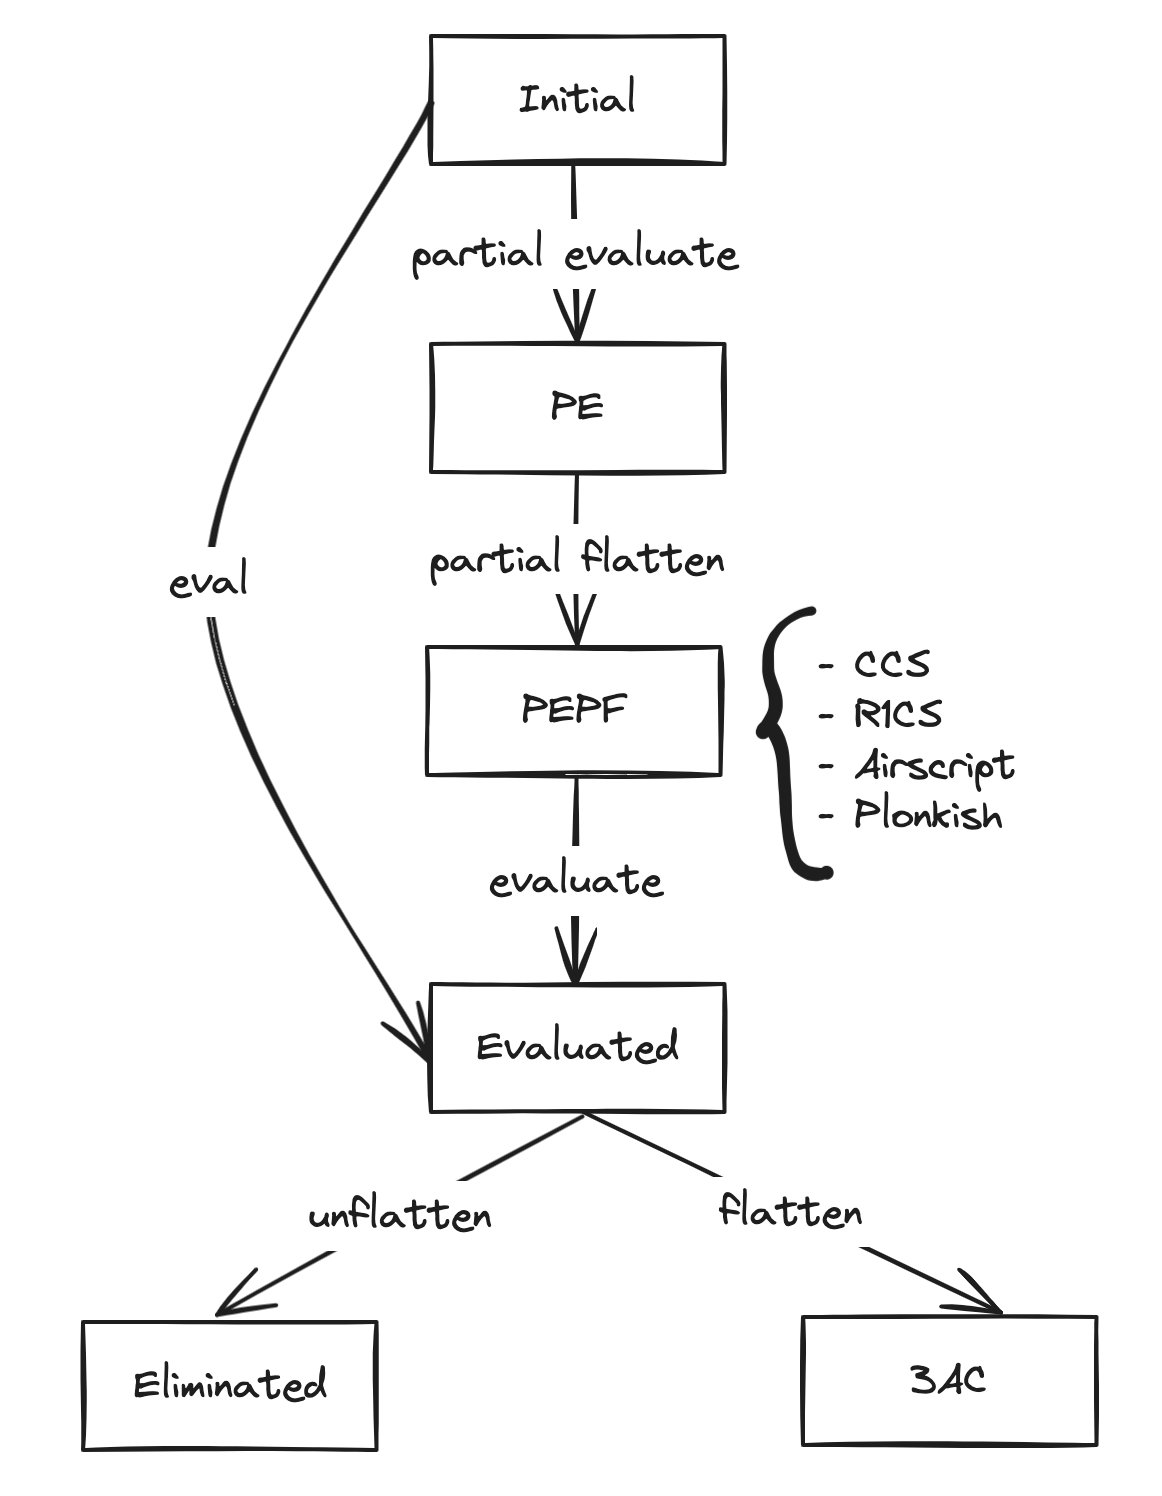
\includegraphics[width=0.5\linewidth]{relationships-diagram.png}
    \caption{Diagram of IR relationships}
    \label{fig:enter-label}
\end{figure}

\subsection{Ideal (simplified) pipeline}

The most widely used IRs are neither fully evaluated nor fully flattened. For example, R1CS and Plonkish may be extended with lookups (unevaluated functions). R1CS has a simple form, but it is still not fully flattened, although its mapping to 3AC is linear. Plonkish has custom gates, thus requiring additional auxiliary data to generate its form.

% 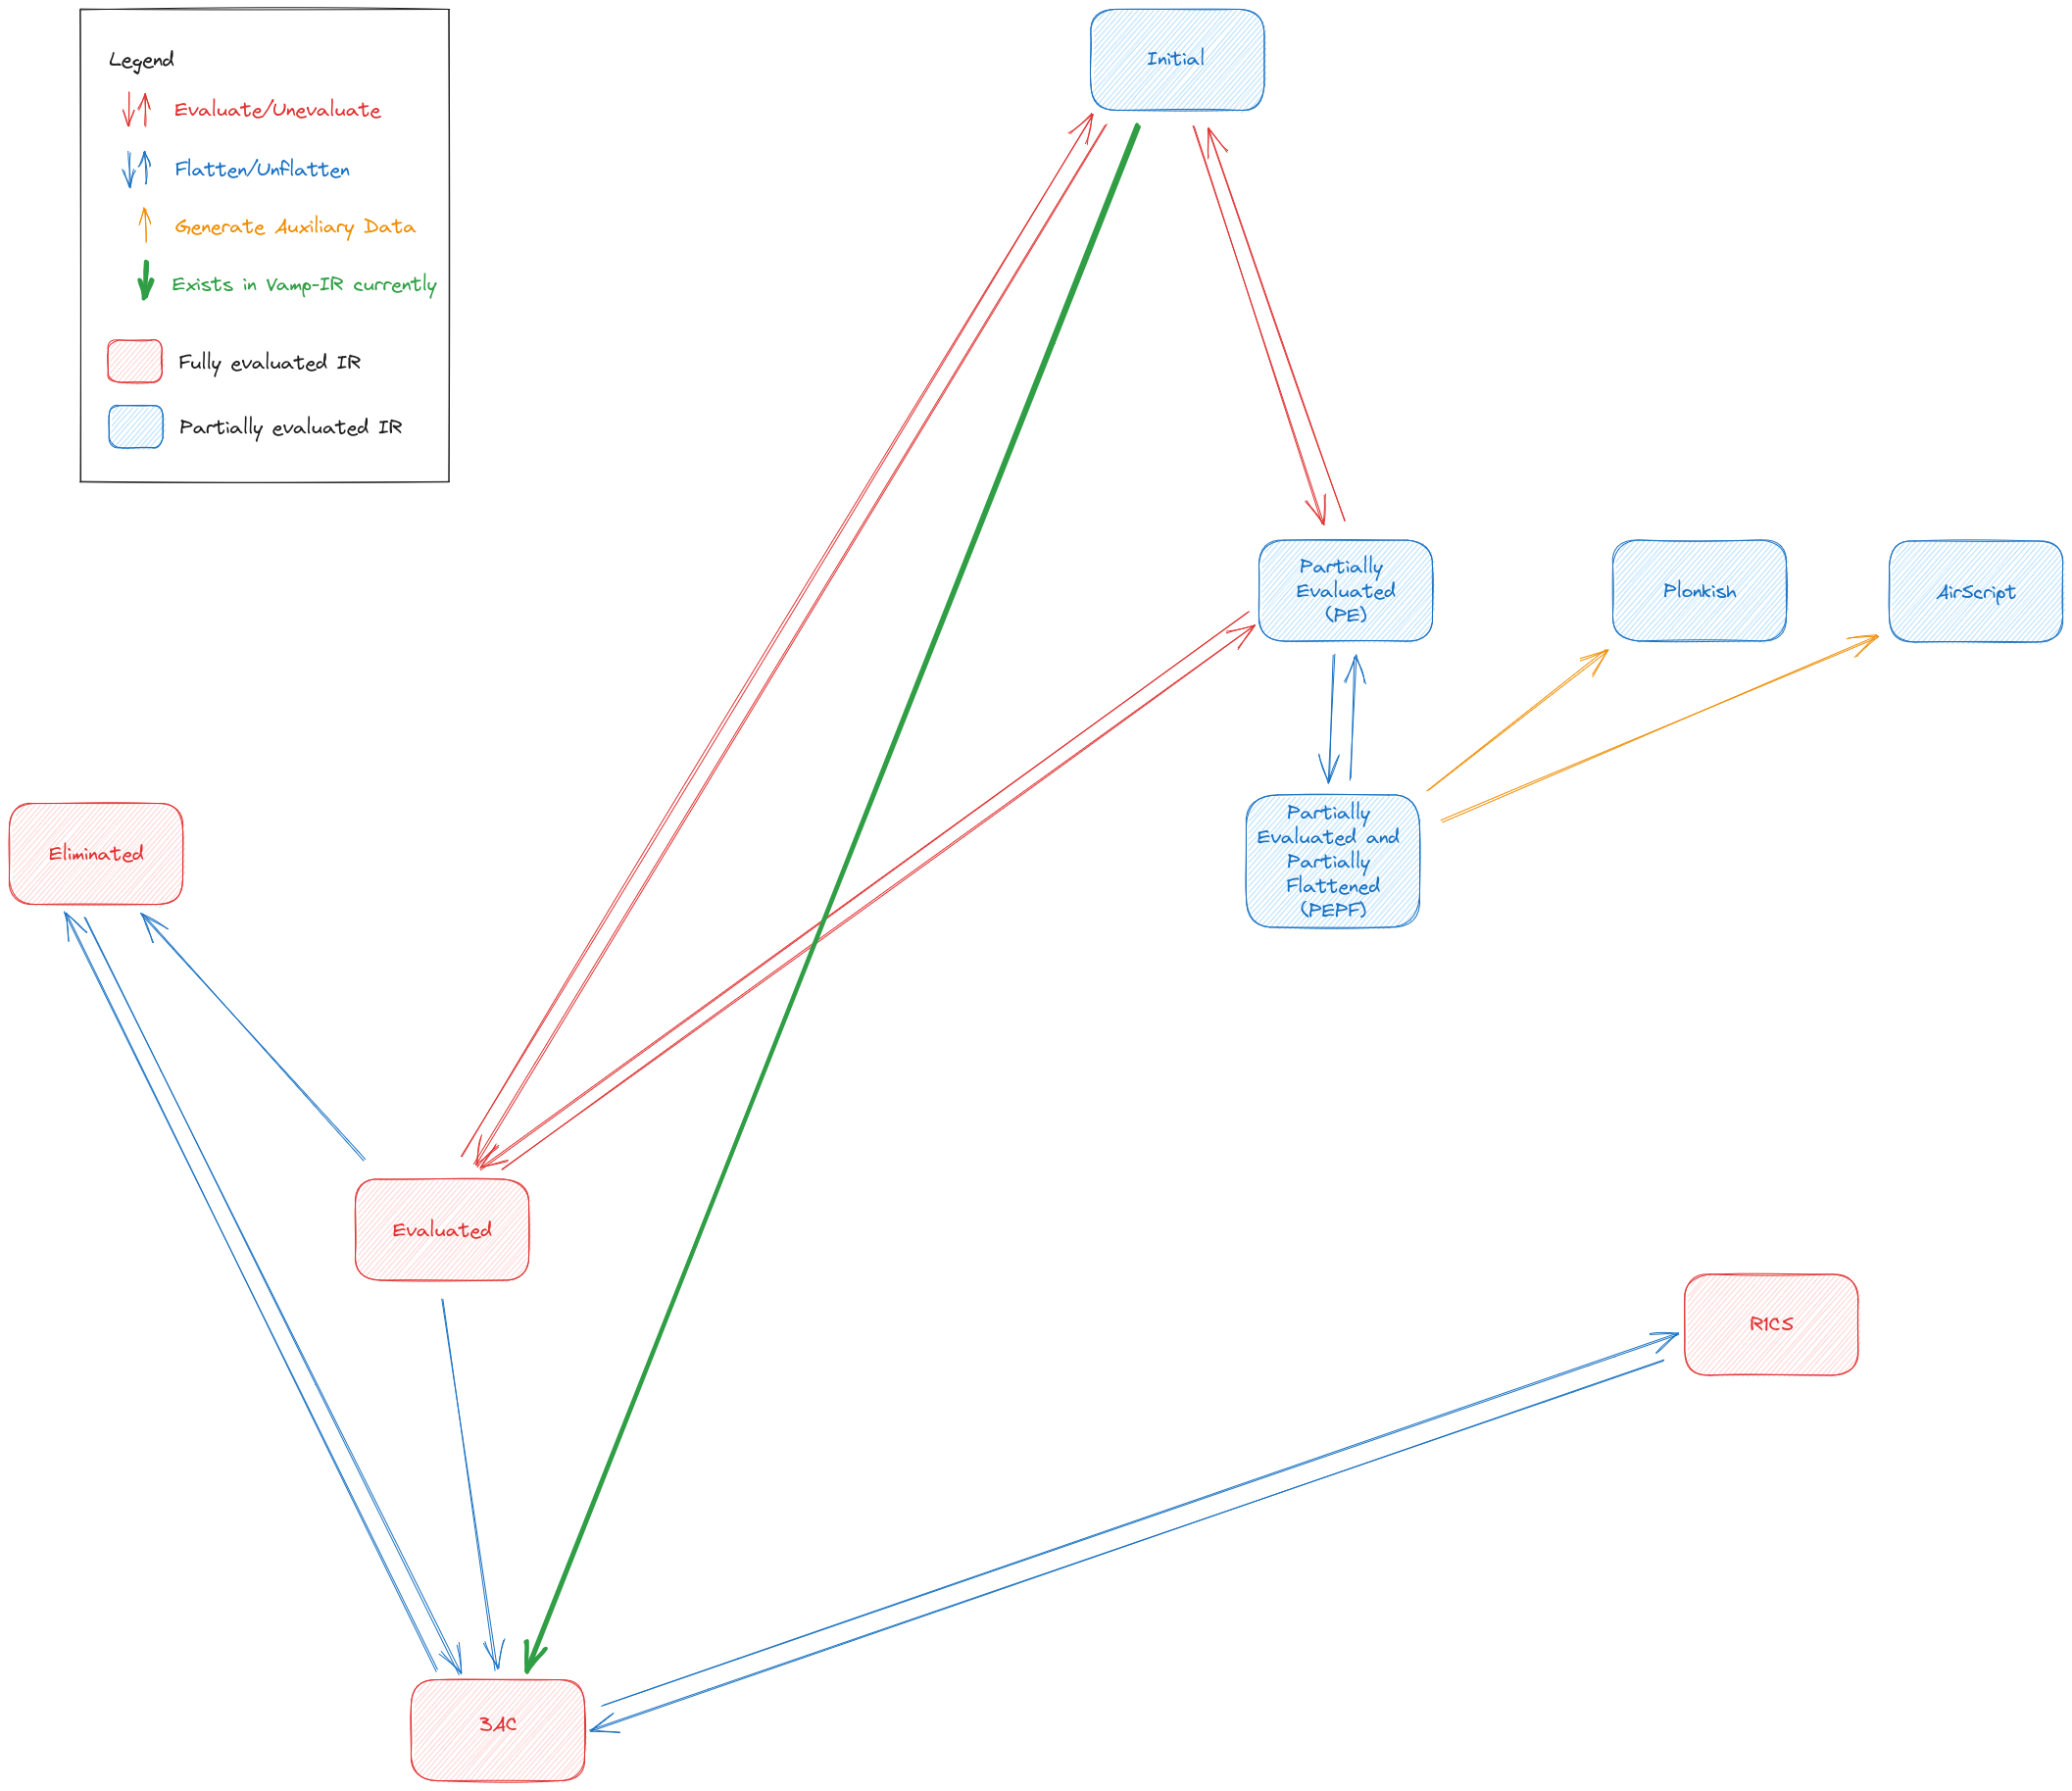
\includegraphics[width=\textwidth]{figs/bestiary-diagram.png}
\begin{figure}[H]
    \centering
    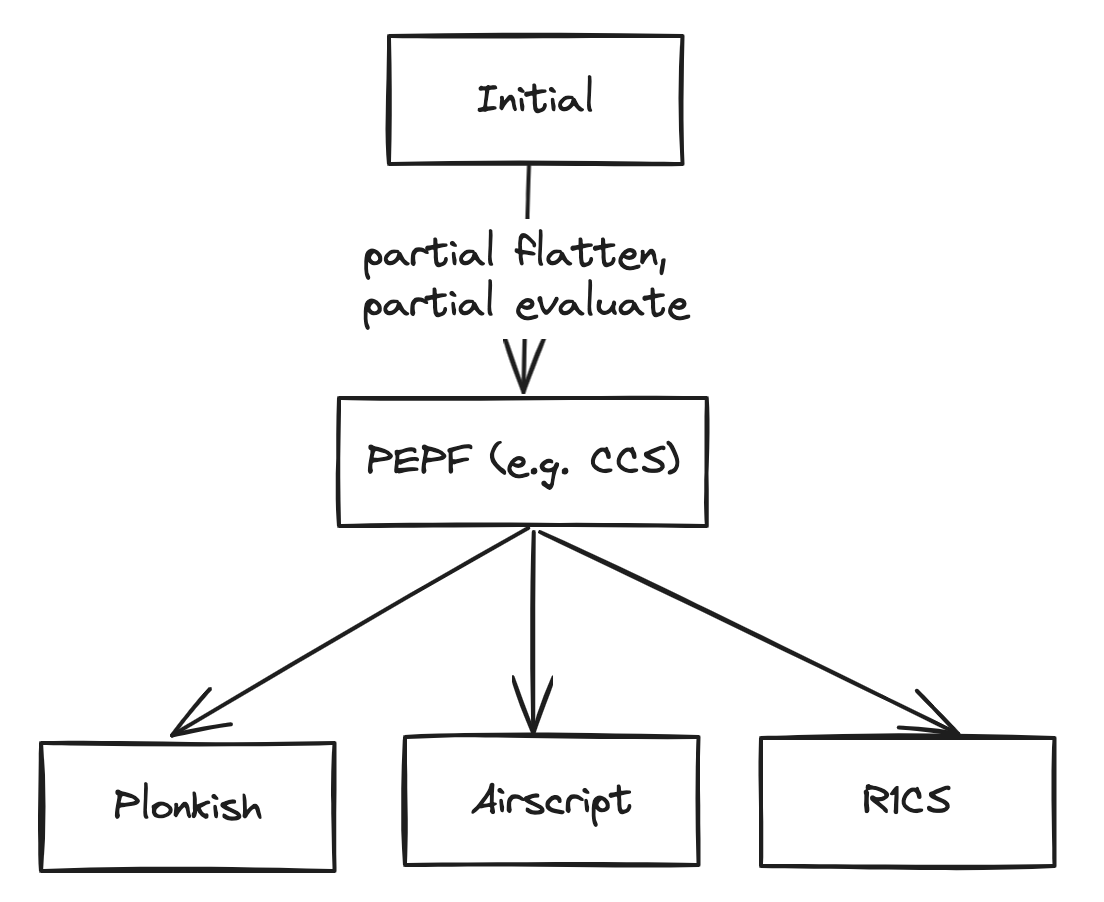
\includegraphics[width=0.5\linewidth]{ideal-pipeline.png}
    \caption{Ideal (simplified) pipeline}
    \label{fig:enter-label}
\end{figure}





\section{Existing Vamp-IRs}

This section analyses the two existing IRs in the current compiler:
\begin{enumerate}
    \item Initial IR
    \item Three-address code (3AC)
\end{enumerate}

\begin{figure}[H]
    \centering
    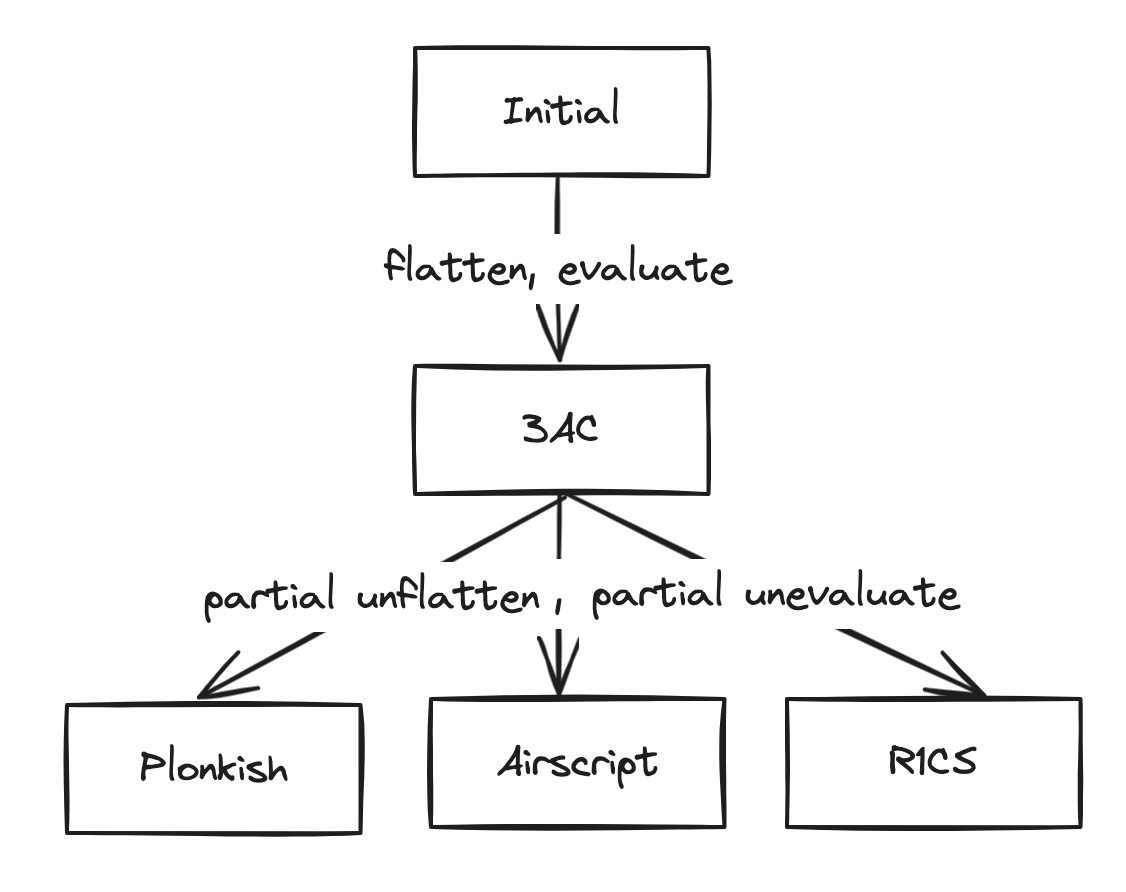
\includegraphics[width=0.5\linewidth]{current-pipeline.png}
    \caption{Current pipeline}
    \label{fig:enter-label}
\end{figure}

\subsection{Initial IR}

After the AST is type-checked we receive a module that retains function calls in its representation and has been only minimally flattened or processed. This IR is close to the initial AST from the parser. This IR has no auxiliary data.

The expression form is a tree whose nodes are labelled with $\text{+, -,}$ or $\times$ and whose leaves are constants, variables, or function calls.

\begin{minted}{python}
Constraint
    = Equal(Variable | Constant, Expr)
    | Equal(Variable | Constant, Function)
    | Equal((Variable | Constant, Variable | Constant, ...), Function)
    
Expr 
    = Add(Expr, Expr) 
    | Subtract(Expr, Expr)
    | Multiply(Expr, Expr)
    | Negate(Expr)
    | Variable
    | Constant
    | Function((Variable | Constant)^k)
\end{minted}

\subsubsection{Example}

\begin{minted}{text}
pubs = [
    c
];

definitions = [
    def is_pyth x y z = {
        def r = (((x^2)+(y^2))-(z^2));
        def r_inv = fresh (1|r);
        (((r*r_inv)-1)*r) = 0;
        r*r_inv
    }
];

constraints = [
    new_score = score + is_pyth a b c;
];

auxiliary_data = [];
\end{minted}

\subsection{Three-address code (3AC)}

\emph{3AC} is totally flattened and totally evaluated. The expression form is either a single node of a tree labelled with $\text{+, -,}$ or $\times$, or is a leaf (i.e. a variable or a constant). Equations are a single, unique, variable on the left and an expression on the right. This IR has no auxiliary data. 

\subsubsection{Description}
Allowed equations:
\begin{align*}
  & z = x + y\\
  & z = x - y\\
  & z = x\times y\\
\end{align*}
  
  ... where $x$, $y$, and $z$ may each be a variable or a constant.

\begin{minted}{text}

Constraint
    = Equal(Variable | Constant, Expr)

Expr 
    = Add(Expr, Variable | Constant) 
    | Subtract(Variable | Constant, Variable | Constant)
    | Multiply(Variable | Constant, Variable | Constant)
    | Negate(Variable | Constant)
    | Variable
    | Constant
\end{minted}

\subsubsection{Example}

\begin{minted}{text}
pubs = [
    c,
];

definitions = [ 
    v1 = a * a,
    v2 = b * b,
    v3 = v1 + v2,
    v4 = c * c,
    v5 = v3 - v4,
    v7 = 1|v5,
    v8 = v7,
    v9 = v5 * v8,
    v10 = v9 - 1,
    v11 = v10 * v5,
    v12 = v5 * v8,
    v13 = score + v12,
];

constraints = [
    v1 = a * a,
    v2 = b * b,
    v3 = v1 + v2,
    v4 = c * c,
    v5 = v3 - v4,
    v8 = v7,
    v9 = v8 * v5,
    v10 = v9 - 1,
    v11 = v10 * v5,
    v12 = v5 * v8,
    v11 = 0,
    new_score = v13,
];

auxiliary_data = [];
\end{minted}


\section{Potential Vamp-IRs}

\subsection{Evaluated}
\emph{Evaluated} is an IR with no remaining function calls, but its expressions may be in any state of flattening.

\subsubsection{Description}

Allowed equations:

  $\displaystyle \quad y = \sum_{i=0}^n\left(c_i\prod_{j=0}^m x_j^{e_{i,j}}\right)$
  
  ... where the $c_i$ are constants, and $y$ and the $x_j$ are variables.

\begin{minted}{text}
Constraint
    = Equal(Variable | Constant, Expr)

Expr 
    = Add(Expr, Expr) 
    | Subtract(Expr, Expr)
    | Multiply(Expr, Expr)
    | Negate(Expr)
    | Variable
    | Constant
\end{minted}

\subsubsection{Example}

\begin{minted}{text}
pubs = [
    c
];

definitions = [
    def v1 = (((x^2)+(y^2))-(z^2)),
    def v2 = fresh (1|v1),
    def v3 = (v1*v2-1)*v1,
    def v4 = v1*v2,
];

constraints = [
    v1 = (((a^2)+(b^2))-(c^2));
    v3 = (v1*v2-1)*v1;
    v4 = v1*v2;
    new_score = score + v4;
    v3 = 0;
];

auxiliary_data = [];
\end{minted}

\subsection{Eliminated}
\emph{Eliminated} form is a maximally unflattened representation with no function calls remaining. All function calls have been evaluated and all unnecessary variables have been eliminated via substitution. The expression form is simply a multivariate polynomial with no restrictions on degree or number of variables. This IR has no auxiliary data. 

Eliminated form is perhaps most useful for human inspection of circuits, say, in LaTeX.

\subsubsection{Description}

Allowed equations:
  
  $\displaystyle \quad y = \sum_{i=0}^n\left(c_i\prod_{j=0}^m x_j^{e_{i,j}}\right)$
  
  ... where the $c_i$ are constants, and $y$ and the $x_j$ are variables.

\begin{minted}{text}
Constraint
    = Equal(Variable | Constant, Expr)

Expr 
    = Add(Expr, Expr) 
    | Subtract(Expr, Expr)
    | Multiply(Expr, Expr)
    | Negate(Expr)
    | Variable
    | Constant
\end{minted}

\subsubsection{Example}

\begin{minted}{text}
pubs = [
    c,
];

definitions = [
    v1 = fresh (1|((a*a + b*b) - (c*c))),
];

constraints = [
    0 = ((a*a + b*b) - (c*c))*v1 - 1) * ((a*a + b*b) - (c*c)),
    new_score = score + ((a*a + b*b) - (c*c))*v1,
];
\end{minted}

\subsection{Partially Evaluated and Partially Flattened (PEPF)}

This is similar to the Initial IR, except that calls to functions not on a "whitelist" have been evaluated, and the arithmetic expressions have undergone some flattening or unflattening. The whitelist forms the auxiliary data in this IR. Expressions retaining white-listed functions have the form:

\texttt{(tuple of outputs) = white\_listed\_fn(inputs)}

An expression not containing a white-listed function will be purely arithmetic with no function calls.

During synthesis, Vamp-IR will replace expressions retaining white-listed functions with an optimized gadget available in the backend. 

\subsubsection{Description}

Allowed expressions:
\begin{align*}
  &y = \sum_{i=0}^n\left(c_i\prod_{j=0}^m x_j^{e_{i,j}}\right)\\
  &y = f(x1, x2, ...)\\
  &(y1, y2, ...) = f(x1, x2, ...)\\
\end{align*}
  
\begin{minted}{text}
Constraint
    = Equal((Variable | Constant)^n, Expr)

Expr 
    = Add(Expr, Expr) 
    | Subtract(Expr, Expr)
    | Multiply(Expr, Expr)
    | Negate(Expr)
    | Variable
    | Constant
    | Function((Variable | Constant)^k)
\end{minted}



\subsubsection{Example}

\begin{minted}{text}
pubs = [
    c
];

definitions = [
    def is_pyth x y z = {
        def r = (((x^2)+(y^2))-(z^2));
        def r_inv = fresh (1|r);
        (((r*r_inv)-1)*r) = 0;
        r*r_inv
    },
];

constraints = [
    v1 = is_pyth a b c
    new_score = score + v1;
];

auxiliary_data = [
    "is_pyth"
];
\end{minted}

\subsection{Plonkish}

\emph{Plonkish} is a family of IRs parameterized by a configuration in its auxiliary data. The configuration in the auxiliary data consists of:
\begin{enumerate}
    \item a list of $k$ fixed columns (also called selectors)
    \item a list of $n$ advice columns (also called witnesses)
    \item a list of $m$ instance columns (also called public inputs)
    \item $D$, the maximum constraint degree
    \item a list of multivariate polynomial constraints (standard and custom gates)
    \item a list of allowed lookup queries (partitions of advice columns)
\end{enumerate}


See more at: \url{https://zcash.github.io/halo2/concepts/arithmetization.html}

Plonkish differs from AIR in that it doesn't require uniform circuits, and unlike R1CS, it can handle constraints of more than a degree of two. This versatility allows Plonkish to depict some program operations more succintly than either R1CS or AIR. However, proving with Plonkish might come at a greater cost per gate or constraint. For many relevant applications, the benefits from smaller circuits could surpass the costs of supporting more expressive gates.

\subsubsection{Description}

Allowed equations:

\begin{align*}
  & custom_{out} = custom(custom_{in})\\
  & lookup_{out} = lookup(lookup_{in})\\ 
\end{align*}

  
...where the $n+m$ advice and instance columns are partitioned into a list of outputs ($custom_{out}$) and a list of inputs ($custom_{in})$ for each custom gate. For lookups, $lookup_{out}$ and $lookup_{in}$ only partition the $n$ advice columns.
  
  Custom gates are multivariate polynomials that must be satisfied by the $k+n+m$ available advice and instance columns, along with a partition of the advice and instance columns into "inputs" and "outputs".
  
  Lookup queries are a partition of the $n$ advice columns into "inputs" and "outputs", much like a function signature. The actual logic of the function is defined elsewhere.
  
\subsubsection{Example}

An example of a circuit using the configuration defined in the auxiliary data. The auxiliary data is given in JSON and defines a configuration with width-5 constraints with a custom gate (\texttt{fifth\_power}) and a lookup gate (\texttt{matrix}).

Notice that some definitions have been written to correspond to the available custom gates and lookups in the configuration. A programmer desiring efficient circuits would write their Vamp-IR code in this manner, but this is not enforced.

This is a 16-bit hash circuit inspired (extremely loosely) by the Poseidon SNARK friendly hash function which uses matrix multiplication and fifth powers.

\begin{minted}{text}
pubs = [];

definitions = [
    def fifth_power x1 = {
        def x2 = x1^5;
        x2
    },
    def matrix x1 x2 = {
        def new_1 = 3*x1 + 7*x2;
        def new_2 = -2*x1 + 5*x2;
        def x3 = range_8 (fresh (new_1 % 2^8));
        def x4 = range_8 (fresh (new_2 % 2^8));
        (x3, x4)
    },
    def bool x = {
        x^2 = x;
        x
    },
    def range_2 x = {
        def lo = bool (fresh (x % 2));
        def hi = bool (fresh (x \ 2));
        x = 2*hi + lo;
        x
    },
    def range_4 x = {
        def lo = range_2 (fresh (x % 2^2));
        def hi = range_2 (fresh (x \ 2^2));
        x = 2^2*hi + lo;
        x
    },
    def range_8 x = {
        def lo = range_4 (fresh (x % 2^4));
        def hi = range_4 (fresh (x \ 2^4));
        x = 2^4*hi + lo;
        x
    },
    def hash_round lo hi = {
        matrix (fifth_power lo) (fifth_power hi)
    }, 
    def hash x = {
        def lo = range_8 (fresh (x % 2^8));
        def hi = range_8 (fresh (x \ 2^8));
        def (new_lo, new_hi) = iter 10 hash_round lo hi;
        2^8*hi_mod + lo_mod
    },
];

constraints = [
    y = hash x,
];

auxiliary_data = {
    "fixed_columns": ["a", "b", "c", "d", "e"],
    "advice_columns": ["x1", "x2", "x3", "x4"],
    "instance_columns": [],
    "D": 5,
    "custom_gates": [
        {
            "standard": {
                "constraint": a*x1*x2 + b*x1 + c*x2 + d*x3 + e*x4",
                "inputs": ["x1", "x2", "x4"],
                "outputs": ["x3"]
            },
            "fifth_power": {
                "constraint": "x2 - x1^5",
                "inputs": ["x1"],
                "outputs" ["x2"]
            },
        }
    ],
    "lookups": [
        {
            "matrix": {
                "inputs": ["x1", "x2"],
                "outputs": ["x3", "x4"]
            }
        } 
    ] 
}
\end{minted}

\subsection{R1CS}

\emph{R1CS} uses constraints of the form $C = A\times B$ where $A$, $B$, and $C$ are \textit{linear combinations} of variables and constants. For convenience, we designate one variable in $C$ to be the "out" variable and write only it on the left. The rest of the terms in $C$ are moved to the right. This IR needs no auxiliary data.

\subsubsection{Formal definition}
Allowed equations:

$\displaystyle z = \left(\sum_{i=0}^n a_i x_i\right)\left(\sum_{i=0}^n b_i x_i\right) - \left(\sum_{i=0}^n c_i x_i\right)$


\subsubsection{Example}

\begin{minted}{text}
pubs = [
    c,
];

definitions = [
    v1 = (2*a)*b,
    v2 = (a + b - c)*(a + b + c) - v1,
    v3 = 1|v2,
    v4 = v2 * v3,   
];

constraints = [
    v1 = (2*a)*b,
    v2 = (a + b - c)*(a + b + c) - v1,
    v4 = v2 * v3,
    0 = (v4 - 1)*v2,
    new_score = v4 + score,
];

auxiliary_data = [];
\end{minted}

\subsection{AirScript}

\emph{AirScript} is an intermediate representation used by PolygonMiden which compiles to the Winterfell STARK proof system. STARKs are very inefficient unless the circuit conforms to certain structure: namely, that the entire circuit can be written as a bounded loop of a relatively small subcircuit.

If a Vamp-IR circuit has this structure it is fairly simple to compile it into AirScript by computing some auxiliary data.

\subsubsection{Auxiliary Data Format}

In order to compile Vamp-IR to AirScript we need:
\begin{enumerate}
    \item a list of private main register names
    \item (optional) a list of private auxiliary register names
    \item at least one public register with a name and a length
    \item a hashmap from Vamp-IR variable names to AirScript register names
    \item every variable in the Vamp-IR document needs to be mapped uniquely to a private or public register name with the appropriate suffix if needed: .first, .last, ')
    \item a partition of the constraints into boundary constraints and integrity constraints
\end{enumerate}


\subsubsection{Generating the Auxiliary Data}
Consider the simple case of an iterated function in Vamp-IR. The function below has the same number of inputs as the outputs and so it works very much like a register machine with registers \textit{a}, \textit{b}, \textit{c}, and \textit{d}. The entire circuit is a single function iterated 8 times, along with some constraints on the initial inputs and final outputs of the function.

\begin{minted}{text}
def my_function (a, b, c, d) = {
  def a_next = a + c;
  def b_next = b + d;
  def c_next = c - 1;
  def d_next = 2*d;
  
  (a_next, b_next, c_next, d_next)
};

(a_out, b_out, c_out, d_out) = iter 8 my_function(a_in, b_in, c_in, d_in);

c_out = 0;
b_in = a_in;
\end{minted}

\begin{enumerate}
    \item Evaluate all function calls within \textit{my\_function}, replacing them with the appropriate constraints and definitions. Do \emph{not} evaluate the intrinsic \textit{iter}.
    \item Condense the constraints within \textit{my\_function} by eliminating all intermediate variables. This will reduce the number of registers we need.
    \item Create a register name as a string for each non-public parameter of \textit{my\_function} and each internal non-public variable in \textit{my\_function}, *excluding the output variable(s)*. Add an entry for each variable to the variable name map.
    \item  Create a register name for each public input accessed by \textit{my\_function}. Pubs are declared globally by name in Vamp-IR so these names should be reused here. A list of these names and the length of each register needed becomes the data in \textit{public\_inputs} above. Add an entry for each public variable to the variable name map. AirScript requires at least one public variable, so if the list of pubs is empty a dummy public variable should be created.
    \item Loop through the list of expressions and add an entry to the partition hashmap for each expression. Boundary constraints will only reference variables mapped to \textit{(register name).first} or \textit{(register name).last}. Integrity constraints will only reference variables mapped to \textit{(register name)} or \textit{(register name)'}. A constraint that references variables from both classes is invalid.
\end{enumerate}


\subsubsection{Example}


\begin{minted}{text}
pubs = [];

definitions = [
    def my_function (a, b, c, d) = {
      def a_next = a + c;
      def b_next = b + d;
      def c_next = c - 1;
      def d_next = 2*d;

      (a_next, b_next, c_next, d_next)
    },
];

constraints = [
    a_next = a + c,
    b_next = b + d,
    c_next = c - 1,
    d_next = 2*d,
    c_out = 0,
    b_in = a_in,
];

auxiliary_data = {
    "main_registers": ["a", "b", "c", "d"],
    "auxregisters": [],
    "public_inputs": ["dummy", 1],
    "variable_mapping": {
        "a": "a",
        "b": "b",
        "c": "c",
        "d": "d",
        "a_in": "a.first",
        "b_in": "b.first",
        "c_in": "c.first",
        "d_in": "d.first",
        "a_out": "a.last",
        "b_out": "b.last",
        "c_out": "c.last",
        "d_out": "d.last",
        "a_next": "a'",
        "b_next": "b'",
        "c_next": "c'",
        "d_next": "d'",
    },
    "periodic_columns": [],
    "constraints": {
        "integrity": [
            "a_next = a + c",
            "b_next = b + d",
            "c_next = c - 1",
            "d_next = 2*d",
        ],
        "boundary": [
            "c_out = 0",
            "b_in = a_in",
        ]
    }
}
\end{minted}

\subsubsection{Compiling more complex Vamp-IR circuits to AirScript}
The scheme above does not make use of \emph{periodic columns}. Periodic columns allow different constraints to be active on different cycles. We can use the periodic columns to allow for more complex Vamp-IR circuits which have some constraints on computation done before or after the iterated function. (Hash functions come to mind as an example of this.)

The scheme above also does not use any \emph{auxiliary trace columns}. Auxiliary trace columns can access new randomness from the Verifier. (Author note: I am not sure what auxiliary trace columns are used for. I suspect they are needed for folding or recursion.)

\subsection{CCS}

\textit{Custom constraint system} or CCS is a new constraint system that generalizes Plonkish, R1CS, and AIR constraints. CCS is more general in the sense there are costless reductions from instances of these IRs to equivalent CCS instances.

A CCS instance consists of public input $x \in \mathbb{F}^l$. A CCS witness consists of a vector $w \in \mathbb{F}^{n-l-1}$. A CCS structure-instance tuple (S, x) is satisfied by a CCS witness w if 
\begin{equation}
    \sum_{i=0}^{q-1} c_i \cdot \circ_{j \in S_i} M_j \cdot z = \mathbf{0}
\end{equation}

where $z = (w, 1, x) \in \mathbb{F}^n$

$M_j \cdot z$ denotes matrix-vector multiplication. $\circ$ denotes the Hadamard product between vectors, and 0 is an m-sized vector with entries equal to the the additive identity in $\mathbb{F}$.

Expanded, this equation looks like:
\begin{equation*}
    c_0 \cdot \overbrace{(M_{j_{0}} \cdot z \circ ... \circ M_{j_{|{S_{0}}|-1}} \cdot z)}^{j_i \in S_0} + ... + c_{q-1} \cdot \overbrace{(M_{j_{0}} \cdot z \circ ... \circ M_{j_{|{S_{q-1}}|-1}} \cdot z)}^{j_i \in S_{q-1}} = \mathbf{0}
\end{equation*}

\begin{definition}[CCS]
    A CCS structure $S$ consists of: 
    \begin{enumerate}
        \item a sequence of matrices $M_0,..., M_{t-1} \in \mathbb{F}^{m\times n}$ with at most $N = \Omega(max(m, n))$ non-zero entries in total. (You can think of these matrices as a generalisation of the $A,B,C$ matrices in R1CS that encode the constraints).
        \item a sequence of q multisets $[S_0,...,S_{q-1}]$, where an element in each multiset is from the domain ${0,..., t-1}$ and the cardinality of each multiset is at most d. (You can think of $S_i$ as containing the pointers to the matrices $M_i$ for each of the addends in the CCS equation).
        \item a sequence of q constants $[c_0,...,c_{q-1}]$, where each constant is from $\mathbb{F}$
        \item size bounds $m, n, N, l, t, q, d \in N$ where $n \ge l$
        \begin{itemize}
            \item $m$ is the number of constraints (i.e. rows in the Plonkish matrix representation)
            \item $n$ is the number of private and public inputs (i.e. columns in the Plonkish matrix representation, excluding selectors)
            \item $N$ is the total number of non-zero entries in $M_0,...,M_{t-1}$
            \item $l$ is the number of public inputs (thus $n-l$ is the number of private inputs)
            \item $t$ is the number of $M$ matrices. (e.g. in R1CS, which can be seen as an instance of CCS, there are 3 $M$ matrices: $A$, $B$ and $C$)
            \item $q$ is the number of addends in the CCS equation (i.e. $q = |\{S_i\}|$)
            \item $d$ is the upper bound of the cardinality of each $S_i$
        \end{itemize}
    \end{enumerate} 
\end{definition}



\subsubsection{Lookups}

The definition of CCS with lookups (CCS+) is exactly as the definition of CCS, with the following two properties
\begin{itemize}
    \item a lookup table $T$ , where $T$ is a set of values from $\mathbb{F}$
    \item a sequence of lookup operations $L$, where each entry in $L$ is in the range $[n]$.
\end{itemize}

and a CCS+ structure-instance tuple (S, x) is satisfied by a CCS+ witness w if $w$ satisfies it as a CCS structure-instance tuple and for each lookup operation $o$ in $L$, $z[o] \in T$.

\subsubsection{Representing R1CS in CCS}

As an example, the R1CS equation, $(A \cdot z) \circ (B \cdot z) - C \cdot z = 0$ can be represented with CCS as
$S_{CCS}=(n,m,N,l,t,q,d,[M_0, M_1, M_2], [S_1, S_2], [c_1, c_2])$ where $m, n, N, l$ are from R1CS and $t=3, q=2, d=2, M_0=A, M_1=B, M_2=C, S_1=\{0,1\}, S_2=\{2\}, c_0=1, c_1 = -1$.

\begin{equation*}
    1 \cdot \overbrace{(A \cdot z \circ B \cdot z)}^{S_0 = \{0,1\}} + (-1) \cdot \overbrace{(C \cdot z)}^{S_1=\{2\}}
\end{equation*}

\subsubsection{Formal definition}
Allowed equations:

\begin{align*}
  & \displaystyle z = \left(\sum_{i=0}^n a_i x_i\right)\left(\sum_{i=0}^n b_i x_i\right) - \left(\sum_{i=0}^n c_i x_i\right) \\
  & lookup_{out} = lookup(lookup_{in})\\ 
\end{align*}


\subsubsection{Example code}

\begin{minted}{text}
pubs = [
    c,
];

definitions = [
    v1 = (2*a)*b,
    v2 = (a + b - c)*(a + b + c) - v1,
    v3 = inverse v2,
    v4 = v2 * v3,   
];

constraints = [
    v1 = (2*a)*b,
    v2 = (a + b - c)*(a + b + c) - v1,
    v4 = v2 * v3,
    0 = (v4 - 1)*v2,
    new_score = v4 + score,
];

auxiliary_data = {
    "lookups": [
        {
            "inverse": {
                "inputs": ["x1"],
                "outputs": ["x2"]
            }
        } 
    ] 
};
\end{minted}


\subsubsection{Representing Plonkish in CCS}

Plonkish circuits are typically described in terms of gate checks, copy checks, permutation checks, etc. and the Plonk proving system is a set of gadgets to prove these types of checks. That is, description of Plonkish re typically closely tied to how the Plonk proof system internally works.

\begin{definition}[Plonkish]
    A Plonkish structure $S$, $S_{Plonkish}=(m,n,l,t,q,d,e,g,T,s)$, consists of:
    \begin{itemize}
        \item a multivariate polynomial $g$ in $t$ variables where $g$ is expressed as a sum of $q$ monomials and each monomial has a total degree at most $d$. That is
        \begin{equation*}
            g(X_1,...,X_t) = \sum_{i=0}^q k_i \cdot X_1^{i_1} ... X_t^{i_t}
        \end{equation*}
        where $i_1 + ... + i_t \leq d$ for all $i$.
        \item a vector of constants called \textit{selectors} $s \in \mathbb{F}^e$
        \item a set of $m$ constraints. Each constraint $i$ is specified via a vector $T_i$ of length $t$, with entries in the range $\{0,...,n+e-1\}$.
        \begin{equation*}
            T_i := [T_{i_0}, ..., T_{i_{t-1}}] \; \text{(constraint)}
        \end{equation*}
        That is, if $j < n-l$, then $T_i[j]$ will be a private input $w_j$. If $j \geq n-l$ and $j < n$, then $T_i[j]$ will be a private input $x_j$. Otherwise, $T_i[j]$ will be a selector.
        \item size bounds $m, n, l, t, q, d, e \in \mathbb{N}$
        \begin{itemize}
            \item $m$ is the number of constraints (i.e. rows in the Plonkish matrix representation)
            \item $n$ is the number of private and public inputs (i.e. columns in the Plonkish matrix representation, excluding selectors)
            \item $l$ is the number of public inputs ($n-l$ is the number of private inputs)
            \item $t$ is the number of variables in the polynomial $g$
            \item $q$ is the number of monomials that compose $g$
            \item $d$ is the maximum degree of $g$
            \item $e$ is the number of selectors
        \end{itemize}
    \end{itemize}
\end{definition}

A Plonkish instance consists of public input $x \in \mathbb{F}^l$. A Plonkish witness consists of a vector $w \in \mathbb{F}^{n-l}$. A Plonkish structure-instance tuple $(S, x)$ is satisfied by a Plonkish witness $w$ if for all $i \in \{ 0,..., m-1\}$,
\begin{equation}
    g(z[T_i[1]], ..., z[T_i[t]]) = 0
\end{equation}
where $z = (w, x, s) \in \mathbb{F}^{n+e}$

How does the Plonkish representation that CCS proposes compare to the existing representation?
Plonkish is often specified with a combination of gate constraints and copy constraints. Plonkish in CCS eschews copy constraints by using a "deduplicated" version of the satisfying assignment whose length is shorter than a Plonkish satisfying assignment by the number of copy constraints.
% TODO: I don't fully understand this "deduplication" explanation

\subsubsection{CCS to Plonkish}
How does the structure of CCS compare to Plonkish?

$S_{Plonkish}=(m,n,l,t,q,d,e,g,T,s)$

$S_{CCS}=(m,n,N,l,t,q,d,[M_0,...,M_{t-1}], [S_0,...,S_{q-1}], [c_0,...,c_{q-1}])$

% In Plonkish, $t$, $q$ and $d$ are properties of a given polynomial $g$. That is, $t$ the number of variables, $q$ the number of addends and $d$ the maximum degree of each monomial. Its constraints are of the form
% \begin{equation*}
%     g(X_1,...,X_t) := \sum_{i=0}^q k_i \cdot X_1^{i_1} ... X_t^{i_t} = 0 
% \end{equation*}

% In CCS, $t$ is not the number of variables of $g$ but the number of matrices $|\{M_i\}|$. However, there are clear similarities, since the CCS constraints can also be seen as $g(M_1,...,M_t) = 0$ where
% \begin{equation*}
%     g(M_1,...,M_t) := \sum_{i=0}^q k_i \cdot ((M_{1} \cdot z)_{i_1} \circ ... \circ (M_{t} \cdot z)_{i_t}) = 0 
% \end{equation*}
% and $(M_{j} \cdot z)_{i_1}$ is either $M_j \cdot z$ or $\mathbf{0}$.

How do we derive $M_0,..., M_{t-1}$?
There is a row for each constraint in $S_{Plonkish}$, so, it suffices to specify how the $i$th row of these matrices is set. 

For all $j \in \{0, 1, ... , t - 1\}$, let $k_j = T_i[j]$ (recall that $t$ is the number of variables in $g$ and $T_i$ represents a constraint in vector form). So $k_j$ is one of the values in a constraint.

If $k_j \geq n$ (i.e. if $k_j$ is greater than the number of public and private inputs - it points to a selector), then we set $M_j[i][0] = s[k_j - n]$. Otherwise, we set $M_j[i][k_j] = 1$. We set $S_{CCS}.N$ to be the total number of non-zero entries in $M_0, ... , M_{t-1}$.

Each $c_i$ in $[c_0,...,c_{q-1}]$ is the coefficient of the $i$th monomial of $g$. For $i \in \{0, 1, ... , q - 1\}$, if the $i$th monomial contains a variable $j$, where $j \in \{0, 1, ... , t - 1\}$, add $j$ to multiset $S_i$ with multiplicity equal to the degree of the variable.
% TODO: I don't fully understand this variable explanation

% TODO: Describe what it would mean to modify VampIR to use CCS, and analyze what impact this would have on compiler pipeline organisation, complexity, and performance

\subsubsection{Considerations on Vamp-IR}

At first glance, we considered R1CS as a good IR candidate, since its transformation to Plonkish is quite straightforward, while the inverse transformation is not so easy. CCS seemed too general to be useful as a \textit{fixed} IR. However, it doesn't have to be fixed.

We propose CCS with lookups (CSS+) as an IR that is parameterised by the user, that is, the user passes the configuration parameters $(m,n,N,l,t,q,d,[M_0,...,M_{t-1}], [S_0,...,S_{q-1}], [c_0,...,c_{q-1}])$ from $S_{CCS}$. These configuration parameters become part of the auxiliary data. As we saw, we can represent R1CS as CCS by setting $t=3, q=2, d=2, M_0=A, M_1=B, M_2=C, S_1=\{0,1\}, S_2=\{2\}, c_0=1, c_1 = -1$. We also saw that CCS can represent different IRs such as Plonkish or Airscript by setting certain configuration parameters.

How does it affect the structure of the code? We want to provide a default configuration and allow the user to change that configuration before compiling. This configuration will be auxiliary data that is carried along the compilation process.

Given the seemingly efficient transformations among CCS configurations, we could take a circuit and transform it into different configurations to figure out the best.
% CCS also opens up the door to finding the most optimal circuit representation of a given program

\subsubsection{Additional thoughts}

Currently, the Vamp-IR compiler only has two IRs and transformations such as evaluation or flattening happen at the same time. For certain backends such as Halo2, some gadgets benefit from \textit{partial} evaluation. On the other hand, a totally flattened circuit such as 3AC is never the most efficient (e.g. circuit size is bigger than in other forms), although in this form, many compiler optimisations can be applied.

% In the configuration, one could state how much to flatten and which functions to evaluate.


% \begin{itemize}
%     \item Pipeline organisation
%     % Considerations
%     In which order IRs come? Does CCS come before Plonkish/R1CS/AIR? Or Plonkish before CCS? Are they all necessary? What would be an ideal pipeline? 
%     % Since CCS is more general than Plonkish, AIR or R1CS, it intuitively makes sense that CCS is an IR prior to the others.
%     \item Complexity
%     How does it affect the structure of the code? 
%     \item Performance
%     How does adding or removing generality affect performance?
% \end{itemize}

\bibliography{ref.bib}

\end{document}
